\documentclass{article}
\usepackage[utf8x]{inputenc}
\usepackage[english,russian]{babel}
\usepackage{multicol}
\usepackage{amsmath}
\usepackage{geometry}
\usepackage{graphicx}
\newgeometry{top=1cm, bottom=1.8cm, left=1.3cm, right=1.5cm}
\setlength\parindent{0pt}
\pagestyle{empty}

\begin{document}

\begin{multicols}{2}
[
\begin{center}
«З\;А\;Д\;А\;Ч\;Н\;И\;К\; К\;В\;А\;Н\;Т\;А»\begin{flushright}23\end{flushright}
\end{center}
]
ного из O на \textit{EF} -- проведем $E'F'$||$EF$ (см. рис. б). Тогда, по доказанному выше, $E'Q' = Q'F'$ и если $K$ -- точка пересечения $Q'A$ с $EF$, то $EK = KF$. Но точка $K$ отлична от $Q$, значит $EQ \neq QF$.\\
\textit{a}\begin{center}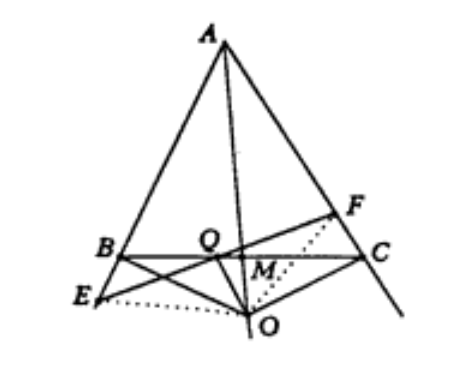
\includegraphics[scale=0.2]{1.png}\end{center}\\
\textit{б}\begin{center}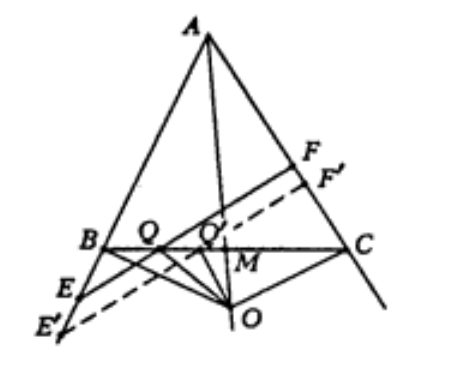
\includegraphics[scale=0.2]{2.png}\end{center}\\
\textit{Замечание.} Рисунок $а$ -- а именно, тот факт, что середина $Q$ основания равнобедренного треугольника  $EOF$ лежит на отрезке $BC$, -- легко объяснить с помощью векторов: поскольку $\overrightarrow{OM} = \left(\overrightarrow{CF} + \overrightarrow{BE}\right)\bigg/2$,\\
$\overrightarrow{OQ} = \left(\overrightarrow{OE} + \overrightarrow{OF}\right)\bigg/2$, то $\overrightarrow{OM} = \left(\overrightarrow{CF} + \overrightarrow{BE}\right)\bigg/2$, а поскольку $\overrightarrow{CF}$ и $\overrightarrow{BE}$ равны по длине, их полусумма направлена по биссектрисе угла между их направлениями.\\\par

М1469. \textit{Для любого целого положительного числа k через f(k) обозначим число всех элементов в множестве \{k+1, k=2, ..., 2k\}, в двоичном представлении каждого из которых имеется в точности три единицы.\\
(а) Докажите, что для каждого целого положительного числа m существует хотя бы одно целое положительное число k такое, что f(k)=m.\\
(b) Найдите все целые положительные числа m, для каждого из которых существует единственное k, удовлетворяющее условию f(k)=m.}\\\par

Пусть $B_k$ -- множество всех чисел от 1 до 2k, в двоичной записи которых ровно 3 единицы, $g(k)$ -- число элементов в $B_k$. Ясно, что $g(k)$ -- неубывающая функция и $f(k) = g(2k) - g(k)$.\par
Поэтому\\
$f(k+1) - f(k) = g(2k+2) - g(k+1) - (g(2k) - g(k)) = $\\
$ = g(2k+2) - g(2k) - (g(k+1)-g(k))$\\
\par
(а) Ясно, что $(2k+2) \in B_{2k+2}$ в том и только в том случае, когда $(k+1)\inB_{k+1}$. Поэтому $f(k+1) - f(k)$ не может
\vfill\null
\columnbreak
\begin{tabular}{|c|c|c|c|c|c|c|c|c|c|c|c|}
    \hline
     & 2 & 3 & 4 & 5 & 6 & 7 & 8 & 9 & 10 & 11 & 12 \\
    \hline
    $g(k)$ & 0 & 0 & 1 & 1 & 2 & 4 & 4 & 4 & 5 & 7 & 7...\\
    \hline
    $f(k)$ & 1 & 2 & 3 & 4 & 5 & 5 & 5 & 6 & 7 & 7 & ...\\
    \hline
\end{tabular}\\\par
вырасти сразу на 2, точнее,
\begin{equation*}
f(k+1) - f(k) = 
 \begin{cases}
   1, &\text{если $(2k+1) \in B_{2k+2}$}
   \\
   0 &\text{в противном случае.}
 \end{cases}
\end{equation*}
Но поскольку, очевидно, $f(k)$ растет неограниченно, эта функция принимает все натуральные значения.\par
(b) Уравнение $f(k)=m$ имеет для некоторого тедин- ственное решение в том и только в том случае, если $f(k+1) - f(k)=1=f(k) - (A(k-1)$ ,т.е. $(2k+1) \in B_{2k+2}$ и оба числа $k$ и $k - 1$ имеют по две единицы в двоичной записи; другими словами, $k = 2^m + 2, n \ge 2$. При этом
$$m=f(2^m +2) = 1+n(n-1)/2 \text{ (где $n=2, 3, … $),}$$
это и есть все нужные, значения m.\\\par
М1470. \textit{Покажите, что существует множество А, состоящее из целых положительных чисел, которое обладает следующим свойством: для каждого бесконечного множества S простых чисел существует k \ge 2, а также существуют два целых положительных числа $m \in \text{А}$ и $n \notin \text{А}$ таких, что оба являются произведениями к различных элементов множества $S$.}\\\par
В качестве А можно взять множество произведений различных простых чисел вида $q_1q_2q_3...q_{q_1}$, где $q_1<q_2<...<q_{q_1}$, (т.е. таких, что число сомножителей равно наименьшему из них: в $А$ входит $2 \cdot 3, 2 \cdot 5, 2\cdot 7,… 3 \cdot 5 \cdot 7, 3 \cdot 5 \cdot 11,…$ и т.д.). Тогда для любого множества $S=\{p_1, p_2, p_3, …\}$ простых чисел, $p_1 < p_2 < p_3 < …$ очевидно, $m=p_2p_3p … p_{p_2}$ входит в $А$, а $n=p_3p_4 … p_{p_2+1}$ не входит в $A$: $p_2 + 1 <  p_3$, а разложение на простые множители единственно («основная теорема арифметики»).\\\par
Ф1478. \textit{С высоты $H = 50$ м без начальной скорости отпускают камень. В тот же момент из точки, находящейся прямо под камнем, начинает удирать по горизонтальной плоскости с постоянной скоростью заяц. При какой минимальной скорости зайца расстояние между ним и камнем в процессе движения не будет уменьшаться?}\\\par
По условию камень падает с ускорением $g$ без начальной скорости, а заяц движется равномерно. Обозначим скорость зайца через $v$. По теореме Пифагора можно выразить расстояние $х$ между зайцем и камнем. Но проще рассматривать квадрат этого расстояния - ведь если положительная величина не уменьшается, то и ее квадрат тоже не уменьшается, а писать лишних корней не придется. Итак,
\begin{align*}
x^2 = \bigg(H - \frac{gt^2}{2}\bigg)^2 + (vt)^2 &= H^2 - Hgt^2 + \frac{g^2t^4}{4} + v^2t^2 = \\
&= H^2 + t^2\bigg(\frac{g^2t^2}{4} + v^2 - gH \bigg)
\end{align*}
    
\end{multicols}

\end{document}
